\documentclass[
    % fontset=ubuntu, % 生僻字可用思源字体,如“昇腾”
    fontset=fandol,
    xcolor=svgnames % SeaGreen
]{ctexbeamer}
\usepackage{pifont} 
\renewcommand{\footnotesize}{\tiny}
\usetheme[
    % compress % 进度条压缩在一行,可选
]{Berlin}
\usepackage{booktabs}
\usecolortheme[named=SeaGreen]{structure}
\usepackage{caption}
\usepackage{float}
\usepackage{subfig}
\usepackage{multirow}
\usepackage{algorithm2e}
\usepackage{xcolor}
\usepackage{graphicx}
\newcommand{\cxmark}{\ding{55}}
\title{可自我诊断异常和优化的人物生成模型}

\subtitle[2024年智能工程学院毕业设计答辩]{
    ~\\
    (2024年智能工程学院毕业设计答辩)
}

\author[方桂安]{
    \texorpdfstring{
        学生:方桂安\\
        ~\\
        \href{mailto: fanggan@mail2.sysu.edu.cn}{fanggan@mail2.sysu.edu.cn}
    }{PDF Bookmark Version}
}

\institute[中山大学~ 智能工程学院(智能科学与技术)]{
    \includegraphics[height=0.1\textheight]{../image/template/logo.png}
    % \includegraphics[height=0.1\textheight]{../image/template/sysu-logo.pdf} % 这里可以放一排所在实验室的logo,可以去学院官网底部或实验室主页弄到,如 <http://nscc-gz.cn/_layout/themes/cs/images/logo0409.png>
}

\logo{\includegraphics[height=0.1\textheight]{../image/template/sysu-logo.pdf}} % 这个是每页都会出现的水印,可能会影响观感,自行决定放不放

\date{
    \today
}

\begin{document}

\section{背景与动机}

\begin{frame}

    \titlepage

\end{frame}

\subsection{选题背景}
\begin{frame}
   \begin{figure}[h]
    \centering
    \includegraphics[width=0.9\textwidth]{fig/intro.pdf}
    \caption{最先进的开源文本到图像生成模型 SDXL 也无法正常生成人物肢体}
    \label{fig:intro}
\end{figure}
\end{frame}
\begin{frame}

    \begin{block}{动机一}
        \begin{itemize}
            \item SDXL\footnote{PODELL D et al. Sdxl: Improving latent diffusion models for highresolution image synthesis[A].}、DALL-E3\footnote{RAMESH A et al. Hierarchical text-conditional image generation
with clip latents: Vol. 1[A].} 以及 DeepFloyd\footnote{SHONENKOV A et al. Deepfloyd if: A
powerful text-to-image model that can smartly integrate text into images[EB/OL].}等模型不断推陈出新
            \item 使用到的预训练数据集规模不断扩大
            \item 在生成高保真度图像领域取得了\alert{显著进步}
        \end{itemize}
    \end{block}

    \begin{block}{动机二}
        \begin{itemize}
            \item HumanSD、ControlNet和T2I-Adapter等工作表现\alert{不尽人意}
            \item 都依赖于额外的输入条件,泛化与应用能力有限
        \end{itemize}
    \end{block}

\end{frame}

\section{概念与挑战}

\subsection{扩散模型}
\begin{frame}
    \begin{figure}[h]
\centering
\includegraphics[width=0.7\linewidth]{figures/diffusion_conditional.pdf}
\caption{有条件扩散模型的整体框架。图像据 \footnote{ROMBACH R et al. High-resolution image synthesis with
latent diffusion models[C]//Proceedings of the IEEE/CVF conference on computer vision and
pattern recognition. } 重现。}
\label{diffusion_conditional}
\end{figure}
\end{frame}
\subsection{T2I-Adapter}
\begin{frame}
    \begin{figure}[h]
\centering
\includegraphics[width=0.95\linewidth]{image/t2iadaper.png}
\caption{T2I-Adapter\footnote{
Chong Mou et al. (2023). T2I-Adapter: Learning Adapters to Dig out More Controllable Ability for Text-to-Image Diffusion Models.
}的原理框架}
\label{diffusion_conditional}
\end{figure}
\end{frame}

\subsection{面临的挑战}

\begin{frame}

    \begin{block}{难点一: 模型}
        \begin{itemize}
            \item 无法即插即用,新模型推出即失效
            \item 
        \end{itemize}
    \end{block}

    \begin{figure}
    \includegraphics[height=0.45\textheight]{../image/humansd.png}
            \caption{HumanSD\footnote{
Ju, X. et al. HumanSD: A Native Skeleton-Guided Diffusion Model for Human Image Generation. arXiv:2304.04269.}}
            \end{figure}
    

\end{frame}
    
            
\begin{frame}

    \begin{block}{难点一: 模型}
        \begin{itemize}
            \item 无法即插即用,新模型推出即失效
            \item 结构复杂,需要额外输入,推理时延增大
        \end{itemize}
    \end{block}

    \begin{figure}
   \includegraphics[height=0.4\textheight]{../image/hyperhuman.png}
            \caption{HyperHuman\footnote{
Liu, X. et al. (2023). HyperHuman: Hyper-Realistic Human Generation with Latent Structural Diffusion. arXiv:2310.08579.
}}
            \end{figure}
    

\end{frame}



\begin{frame}

    \begin{block}{难点二: 数据}
        \begin{itemize}
            \item 现有数据规模小,标注粗糙,缺乏对肢体细节的关注
        \end{itemize}
    \end{block}

    \begin{figure}
   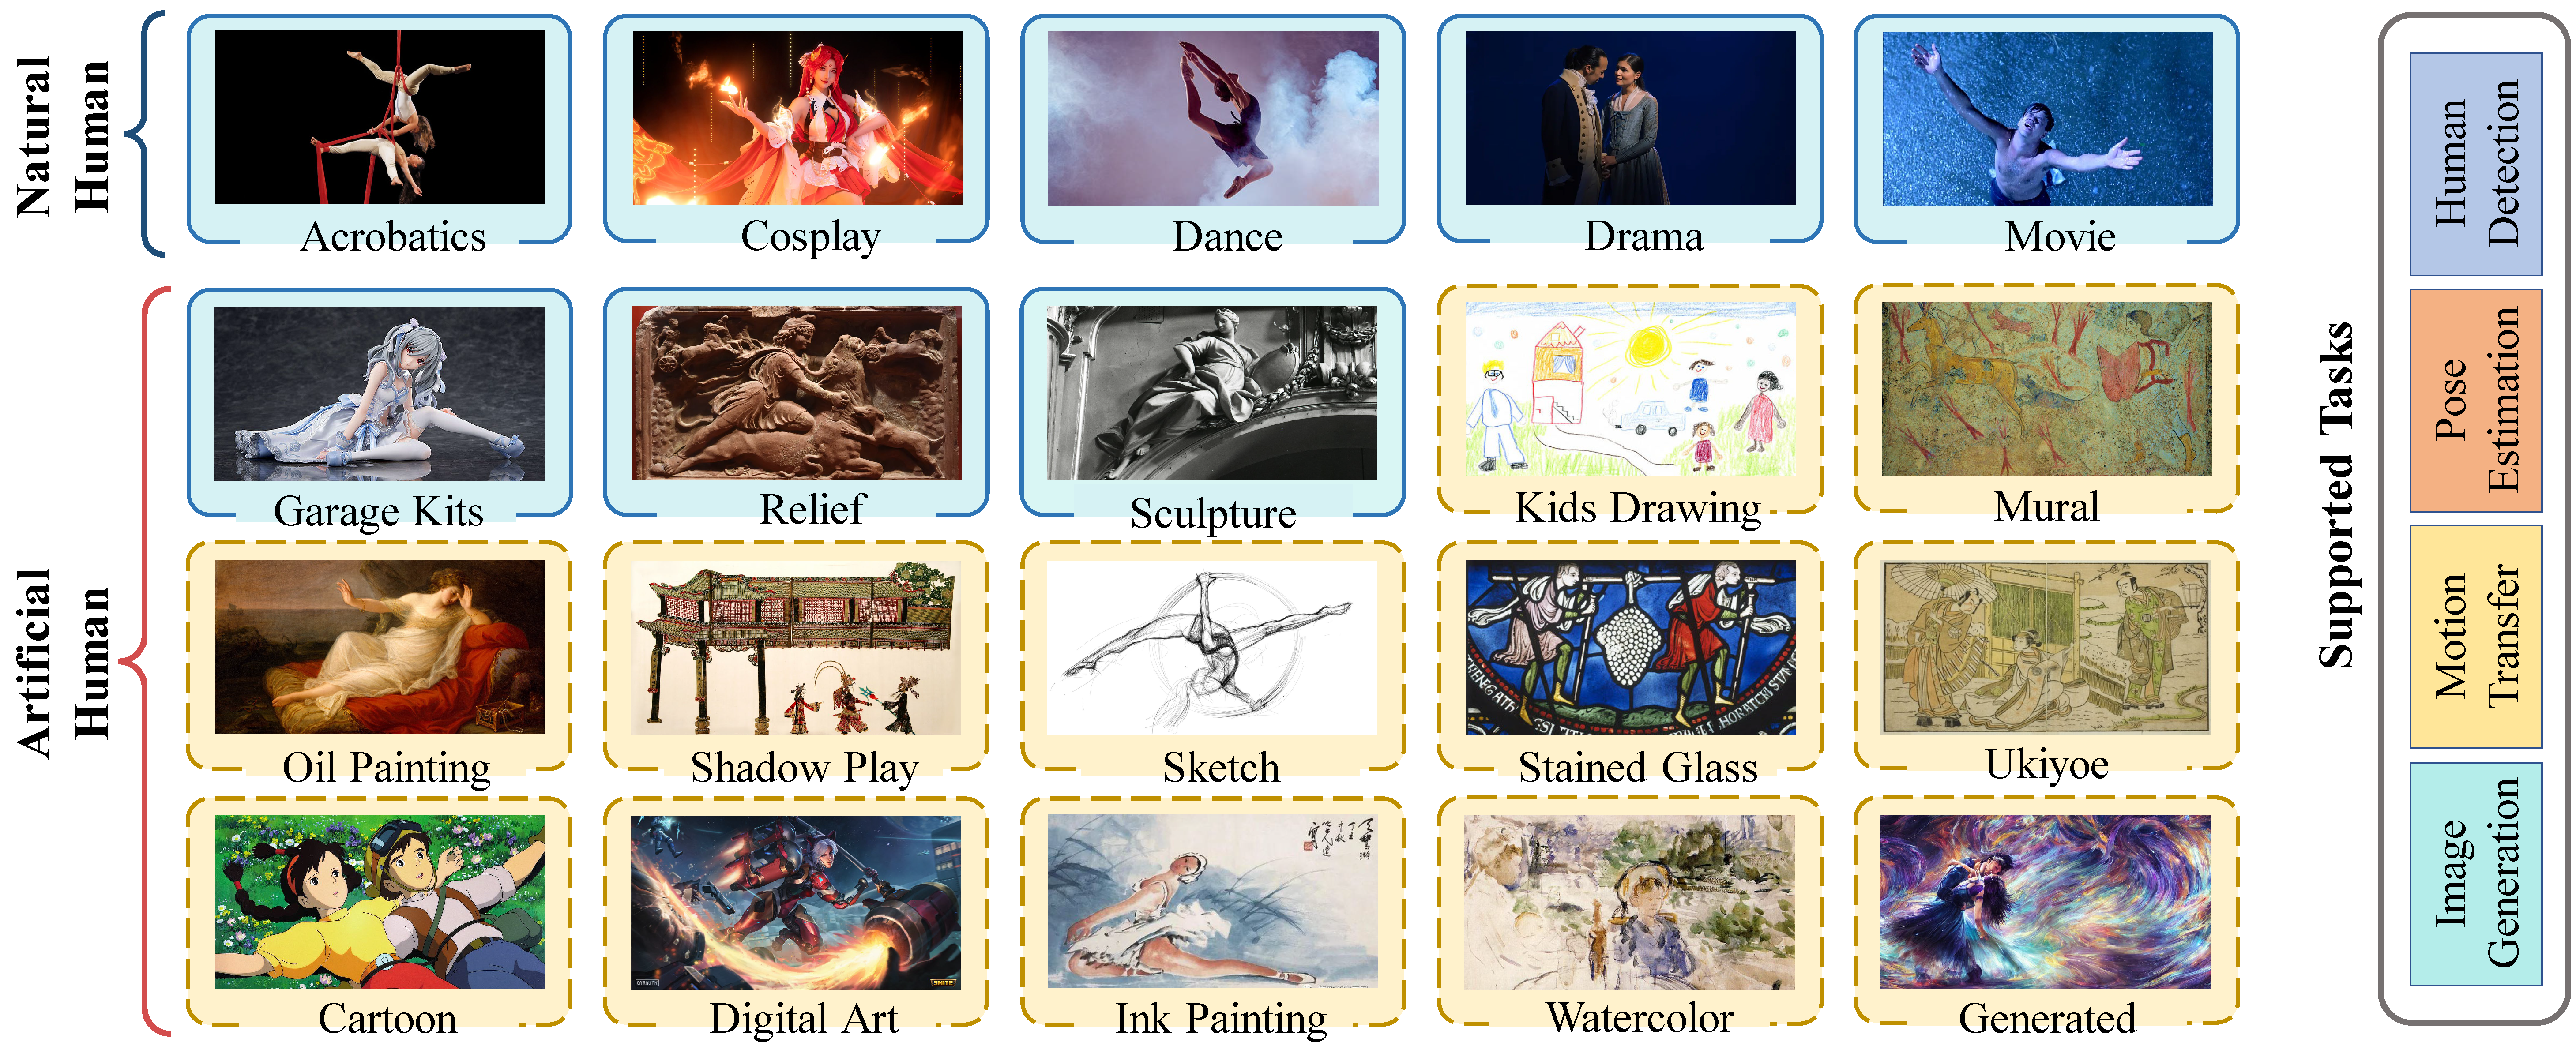
\includegraphics[height=0.45\textheight]{../image/dataset_overview.png}
            \caption{Human-Art\footnote{
Ju, X.et al. (2023). Human-Art: A Versatile Human-Centric Dataset Bridging Natural and Artificial Scenes. In Proceedings of the IEEE/CVF Conference on CVPR.}}
            \end{figure}
    

\end{frame}

% \begin{frame}

%     \begin{block}{要点一}
%         \begin{itemize}
%             \item 条目一
%             \item 条目二
%         \end{itemize}
%     \end{block}

%     \begin{figure} %文中的Grid-LSTM模型做的语义图像分割的例子
%         \includegraphics[width=.2\textwidth,height=.15\textwidth]{../image/chap04/example/2007_000799.jpg}
%         \includegraphics[width=.2\textwidth,height=.15\textwidth]{../image/chap04/example/2007_002094.jpg}
%         \includegraphics[width=.2\textwidth,height=.15\textwidth]{../image/chap04/example/2007_004483.jpg}
%         \includegraphics[width=.2\textwidth,height=.15\textwidth]{../image/chap04/example/2007_003194.jpg}
%         \\
%         \includegraphics[width=.2\textwidth,height=.15\textwidth]{../image/chap04/example/2007_000799.pdf}
%         \includegraphics[width=.2\textwidth,height=.15\textwidth]{../image/chap04/example/2007_002094.pdf}
%         \includegraphics[width=.2\textwidth,height=.15\textwidth]{../image/chap04/example/2007_004483.pdf}
%         \includegraphics[width=.2\textwidth,height=.15\textwidth]{../image/chap04/example/2007_003194.pdf}
%         \caption{并排的多张图像}
%         \label{fig:multi-image-example1}
%     \end{figure}

% \end{frame}

% \subsection{单页双图}

% \begin{frame}

%     \begin{block}{要点一}
%         \begin{itemize}
%             \item 条目一
%             \item 条目二
%         \end{itemize}
%     \end{block}

%     \begin{figure}
%         \begin{minipage}{0.49\textwidth}
%             \includegraphics[height=0.45\textheight]{../image/chap04/example/2007_004483.pdf}
%             \caption{一}
%         \end{minipage}
%         \begin{minipage}{0.49\textwidth}
%             \includegraphics[height=0.45\textheight]{../image/chap04/example/2007_003194.pdf}
%             \caption{二}
%         \end{minipage}
%     \end{figure}

% \end{frame}


\section{设计与实现}

\subsection{合成人像异常肢体数据集}

\begin{frame}

    \begin{block}{AbHuman}
        \begin{itemize}
            \item 提示收集:Laion-5B、Human-Art和 ChatGPT
            \item 图像生成:采用SDXL来生成文本对应的图像
            \item 异常注释:采用 ResNet50 过滤,并标注和评估、复审
            \item 数据分割:分为 52k 训练集和 13k 测试集,以及 200 张高难度的验证集
        \end{itemize}
    \end{block}
\begin{figure}
    \includegraphics[width=1\columnwidth]{fig/dataset_pipeline.pdf}
            \caption{数据集的生成流程}
            \end{figure}


\end{frame}

\subsection{统计与分析}
\begin{frame}

    \begin{block}{AbHuman}
        \begin{itemize}
            \item 识别出了\textbf{ 18 个}
不同的检测类别(例如,正常人类、异常头部、异常颈部、异常身体、异常手臂、
异常手...)
        \end{itemize}
    \end{block}
\begin{figure}
    \includegraphics[width=0.95\columnwidth]{fig/Data_Anno1.pdf}
            \caption{非正常人类注释统计}
            \end{figure}
\end{frame}

\begin{frame}

    \begin{block}{AbHuman}
        \begin{itemize}
            \item AbHuman 提供了\textbf{更细粒度}的注释框和信息,以解决人类生成中的异常问题。
        \end{itemize}
    \end{block}

\begin{table}[htb]
\scriptsize
  \centering
  \caption{以人类为主题的数据集比较,包括人类生成和检测任务。}
    \begin{tabular}{lcccccc}
      \toprule
      数据集 & 图像数量 & 边界框  & 正常 & 异常肢体 & 通用 \\
      \midrule
      BodyHands & 20K   & \checkmark     & \checkmark     & \cxmark     & \cxmark \\
      CrowdPose & 20K   & \checkmark     & \checkmark     & \cxmark     & \cxmark \\
      Multi-Person PoseTrack & 23K   & \checkmark     & \checkmark     & \cxmark     & \cxmark \\
      PoseTrack & 23K   & \checkmark     & \checkmark     & \cxmark     & \cxmark \\
      ClassArch & 1.5K  & \checkmark     & \checkmark     & \cxmark     & \cxmark \\
      Human-Art & 50K   & \checkmark     & \checkmark     & \cxmark     & \checkmark \\
      \midrule
      AbHuman (本文的) & 56K & \checkmark & \checkmark & \checkmark & \checkmark \\
      \bottomrule
    \end{tabular}
  \label{tab:addlabel}
\end{table}
\end{frame}

\subsection{HumanRefiner算法}


\begin{frame}

    \begin{alertblock}{异常评分器}
        \begin{itemize}
            \item 解决了\textbf{缺乏有效的衡量生成图像中肢体质量的标准}问题
        \end{itemize}
    \end{alertblock}
\begin{figure}
    \includegraphics[width=0.8\linewidth]{fig/abnormal-score-visualize.pdf}
    \caption{\textcolor{red}{红色}表示异常分数高的图像,而\textcolor{green}{绿色}表示异常分数低的图像。}

            \end{figure}
\end{frame}

\begin{frame}

    \begin{alertblock}{异常检测器}
        \begin{itemize}
            \item 为了\textbf{精确而高效地定位和识别}人类图像中出现的异常肢体
        \end{itemize}
    \end{alertblock}
\begin{figure}
   
    \includegraphics[width=1\columnwidth]{fig/grid_images_resized.pdf}
    \caption{红色框和标签用于注释检测到的异常肢体,白色用于正常肢体。}
            \end{figure}
\end{frame}
\begin{frame}

    \begin{alertblock}{AbHuman}
        \begin{itemize}
            \item 用负面提示训练的文本到图像扩散模型
            \item 生成的图像通过姿态引导生成全局修正
            \item 通过检测器引导的修补进行局部修正
        \end{itemize}
    \end{alertblock}
\begin{figure}
    \includegraphics[width=1.0\linewidth]{fig/framework_v3.drawio.pdf}\vspace{-3mm}
    \caption{通过提出的AbHuman基准加强的本文的HumanRefiner流程概览。}
            \end{figure}
\end{frame}


\section{实验与结果}
\subsection{定量实验}
\begin{frame}

    \begin{block}{测试结果}
        \begin{itemize}
            \item HumanRefiner 在减少异常、保持内容相关性以及提高图像质量方面具
有较强的能力
        \end{itemize}
    \end{block}

    \begin{table}
\centering
\caption{在AbHuman完整测试集(来自LAION的提示)和困难测试集(来自HumanArt的提示)上的异常分数、CLIP分数和FID分数。}
\resizebox{1\columnwidth}{!}{
\begin{tabular}{c|ccc|ccc}
\toprule
数据集 & \multicolumn{3}{c|}{LAION} & \multicolumn{3}{c}{HumanArt}\\
\hline
模型              & 异常分数$\downarrow$ & CLIP分数$\uparrow$& FID分数$\downarrow$ & 异常分数$\downarrow$ & CLIP分数$\uparrow$ &  FID分数$\downarrow$ \\ \hline
SSD-1B  & 0.612 & 34.02& 16.465 & 0.832 & {33.37} & 13.304 \\
PixArt-XL-2-1024-MS & 0.701 & 34.32& 19.604 & 0.807 & 32.68 & 15.452\\
DeepFloyd-IF & 0.595 & 32.72& 25.926 & 0.849 & 32.67 &21.512\\
LCM  & 0.644 & 32.99& 25.175 & 0.831 & 32.40 & 21.179\\
SDXL & 0.659 & 34.13& 30.024 & 0.857 & 32.40 & 20.796\\
Pose-ControlNet & 0.663 & 33.51& 15.368 & 0.838 & 31.88 & 13.047\\
Pose-T2I-Adapter & 0.624 &  34.79 & 15.658 & 0.807 & 32.72 &12.582\\
HumanSD & 0.661 & 33.78& 50.546 & 0.801 & 33.03 & 38.032\\
HumanRefiner(本文的) & \textbf{0.590} & \textbf{34.85}& \textbf{13.634} & \textbf{0.778} & \textbf{33.90} &\textbf{9.145}\\
\bottomrule
\end{tabular}}
\label{tab:quantitative}
\end{table}

\end{frame}
\subsection{定性实验}
\begin{frame}
\begin{figure}[htb]
	\centering  %图片全局居中
	\subfloat[运动, 一位穿着休闲装的年轻BMX骑手在滑板公园中腾空而起]{
		\includegraphics[width=0.95\linewidth]{fig/316.png}} \\
	\subfloat[战斗, 一位为彩弹比赛装备好的玩家正在森林中前进]{
		\includegraphics[width=0.95\linewidth]{fig/368.png}}
\end{figure}
\end{frame}

\begin{frame}
\begin{figure}[htb]
	\centering  
	\subfloat[瑜伽, 两个人在日落时分的沙滩上表演瑜伽姿势]{
		\includegraphics[width=0.95\linewidth]{fig/370.png}} \\
	\subfloat[舞蹈, 一位穿着白色连衣裙的芭蕾舞者站在墙前]{
		\includegraphics[width=0.95\linewidth]{fig/ap4.png}}
\end{figure}
\end{frame}

\section{总结与展望}
\begin{frame}
     \begin{block}{当前挑战}
        \begin{enumerate}
            \item 推理速度受限
            \item 数据集场景覆盖不全
        \end{enumerate}
    \end{block}

    \begin{alertblock}{未来研究方向}
        \begin{itemize}
            \item 提升文本指导精度与灵活性
            \item 开发轻量化模型与加速策略
            \item 结合3D技术提升真实感
        \end{itemize}
    \end{alertblock}

    \begin{examples}
        \begin{itemize}
            \item 助力在虚拟现实、影视制作、游戏开发等场景中的广泛应用
        \end{itemize}
    \end{examples}
\end{frame}

\begin{frame}
     \begin{block}{重要参考文献}
     \scriptsize
        \begin{enumerate}
           \item PODELL D et al. Sdxl: Improving latent diffusion models for high-resolution image synthesis[A].
           \item SHONENKOV A et al. Deepfloyd if: A powerful text-to-image model that can smartly integrate text into images[EB/OL].
           \item RAMESH A et al. Hierarchical text-conditional image generation with clip latents: Vol. 1[A].
           \item ROMBACH R et al. High-resolution image synthesis with latent diffusion models[C]//Proceedings of the IEEE/CVF conference on computer vision and pattern recognition.
           \item Chong Mou et al. (2023). T2I-Adapter: Learning Adapters to Dig out More Controllable Ability for Text-to-Image Diffusion Models.
           \item Ju, X. et al. HumanSD: A Native Skeleton-Guided Diffusion Model for Human Image Generation. arXiv:2304.04269.
           \item Liu, X. et al. (2023). HyperHuman: Hyper-Realistic Human Generation with Latent Structural Diffusion. arXiv:2310.08579.
           \item Ju, X.et al. (2023). Human-Art: A Versatile Human-Centric Dataset Bridging Natural and Artificial Scenes. In Proceedings of the IEEE/CVF Conference on CVPR.
        \end{enumerate}
    \end{block}
\end{frame}
     

\section{Q \& A}

\begin{frame}

    \begin{block}{Questions?}
        ~\\
        ~\\
        \center{\Huge{Thank you!}}\\
        ~\\
        ~\\
        ~\\
        ~\\
    \end{block}

\end{frame}
\end{document}